\documentclass[aspectratio=169,11pt]{beamer}
\usepackage{iftex}
\ifPDFTeX
  \usepackage[utf8]{inputenc}
  \usepackage[T1]{fontenc}
\else
  \usepackage{fontspec}
  \usepackage{xeCJK}
  \setmainfont{Latin Modern Sans}
  \setsansfont{Latin Modern Sans}
  \setCJKmainfont{FandolSong-Regular}
\fi
\usepackage{graphicx}
\usepackage{booktabs}
\usepackage{array}
\usepackage{hyperref}

\usetheme{Madrid}
\usecolortheme{default}
\definecolor{PrimaryBlue}{RGB}{17,82,147}
\definecolor{AccentBlue}{RGB}{45,117,191}
\setbeamercolor{structure}{fg=PrimaryBlue}
\setbeamercolor{title}{fg=white,bg=PrimaryBlue}
\setbeamercolor{frametitle}{fg=white,bg=PrimaryBlue}
\setbeamercolor{block title}{fg=white,bg=PrimaryBlue}
\setbeamercolor{block body}{fg=black,bg=blue!4}
\setbeamercolor{itemize item}{fg=AccentBlue}
\setbeamerfont{title}{series=\bfseries,size=\Large}
\setbeamerfont{frametitle}{series=\bfseries,size=\large}
\setbeamertemplate{navigation symbols}{}
\setbeamertemplate{headline}{}
\setbeamertemplate{footline}[frame number]

\title[Red Team Testing]{Red Team Testing for Recommendation Systems\\Driven by Large Language Models}
\subtitle{Design and Evaluation of Rag-Poison-Lab}
\author[Sbaaoui Idriss]{Sbaaoui Idriss\\Student ID: 22060004}
\institute[ECUST]{Computer Science, 华东理工大学\\Supervisor: 张恒润}
\date{}

\begin{document}

\begin{frame}[plain]
  \titlepage
\end{frame}

\begin{frame}{Presentation Overview}
\begin{itemize}
  \item Problem and motivation in LLM-driven recommendation pipelines.
  \item Harmful retrieval poisoning threat model.
  \item Rag-Poison-Lab workflow: baseline vs attacked comparison.
  \item Related work supporting recommender poisoning and RAG poisoning.
  \item Technical route: metrics, attacks, and experiment pipeline.
  \item Experimental environment: Docker, backend, Elasticsearch, Kibana, LLM re-ranking.
  \item Sustainability and budget plan.
  \item Thesis schedule.
\end{itemize}
\end{frame}

\begin{frame}{Abstract and Core Motivation}
\begin{itemize}
  \item LLMs are now part of many recommendation pipelines for retrieval, re-ranking, and explanation generation.
  \item This proposal studies \textbf{Red-Teaming Large Language Model-Powered Recommendation Systems}.
  \item The thesis system is Rag-Poison-Lab, built to track poisoning signals from retrieval to final output.
  \item Evaluation uses HR@K, NDCG@K, MRR@K, ASR@K, candidate overlap, and target-rank lift.
  \item Main question: where can an actor attack earliest, and how much can final output be manipulated?
\end{itemize}
\end{frame}

\begin{frame}{Research Background: RAG-Based Recommendation Systems}
\begin{itemize}
  \item The thesis is built around Rag-Poison-Lab with fixed user request and two retrieval modes.
  \item User profile is converted to a retrieval query, candidates are retrieved from Elasticsearch, and top-$K$ items are ranked.
  \item If retrieval changes, final model behavior also changes in RAG pipelines.
  \item The system supports both deterministic ranking and LLM re-ranking for direct comparison.
  \item Dataset: MovieLens 100K, chosen for benchmark quality and local reproducibility.
\end{itemize}
\end{frame}

\begin{frame}{Threat Model: Harmful Retrieval Poisoning}
\begin{itemize}
  \item The attacker does not need to retrain the model.
  \item The attacker can poison indexed data to push intended retrieval candidates.
  \item This can shift ranked output and recommendation explanations.
  \item Planned attack types in the codebase:
  \begin{itemize}
    \item Targeted promotion
    \item Prompt injection payload insertion
    \item Untargeted degradation
  \end{itemize}
\end{itemize}
\end{frame}

\begin{frame}{Rag-Poison-Lab Architecture}
  \centering
  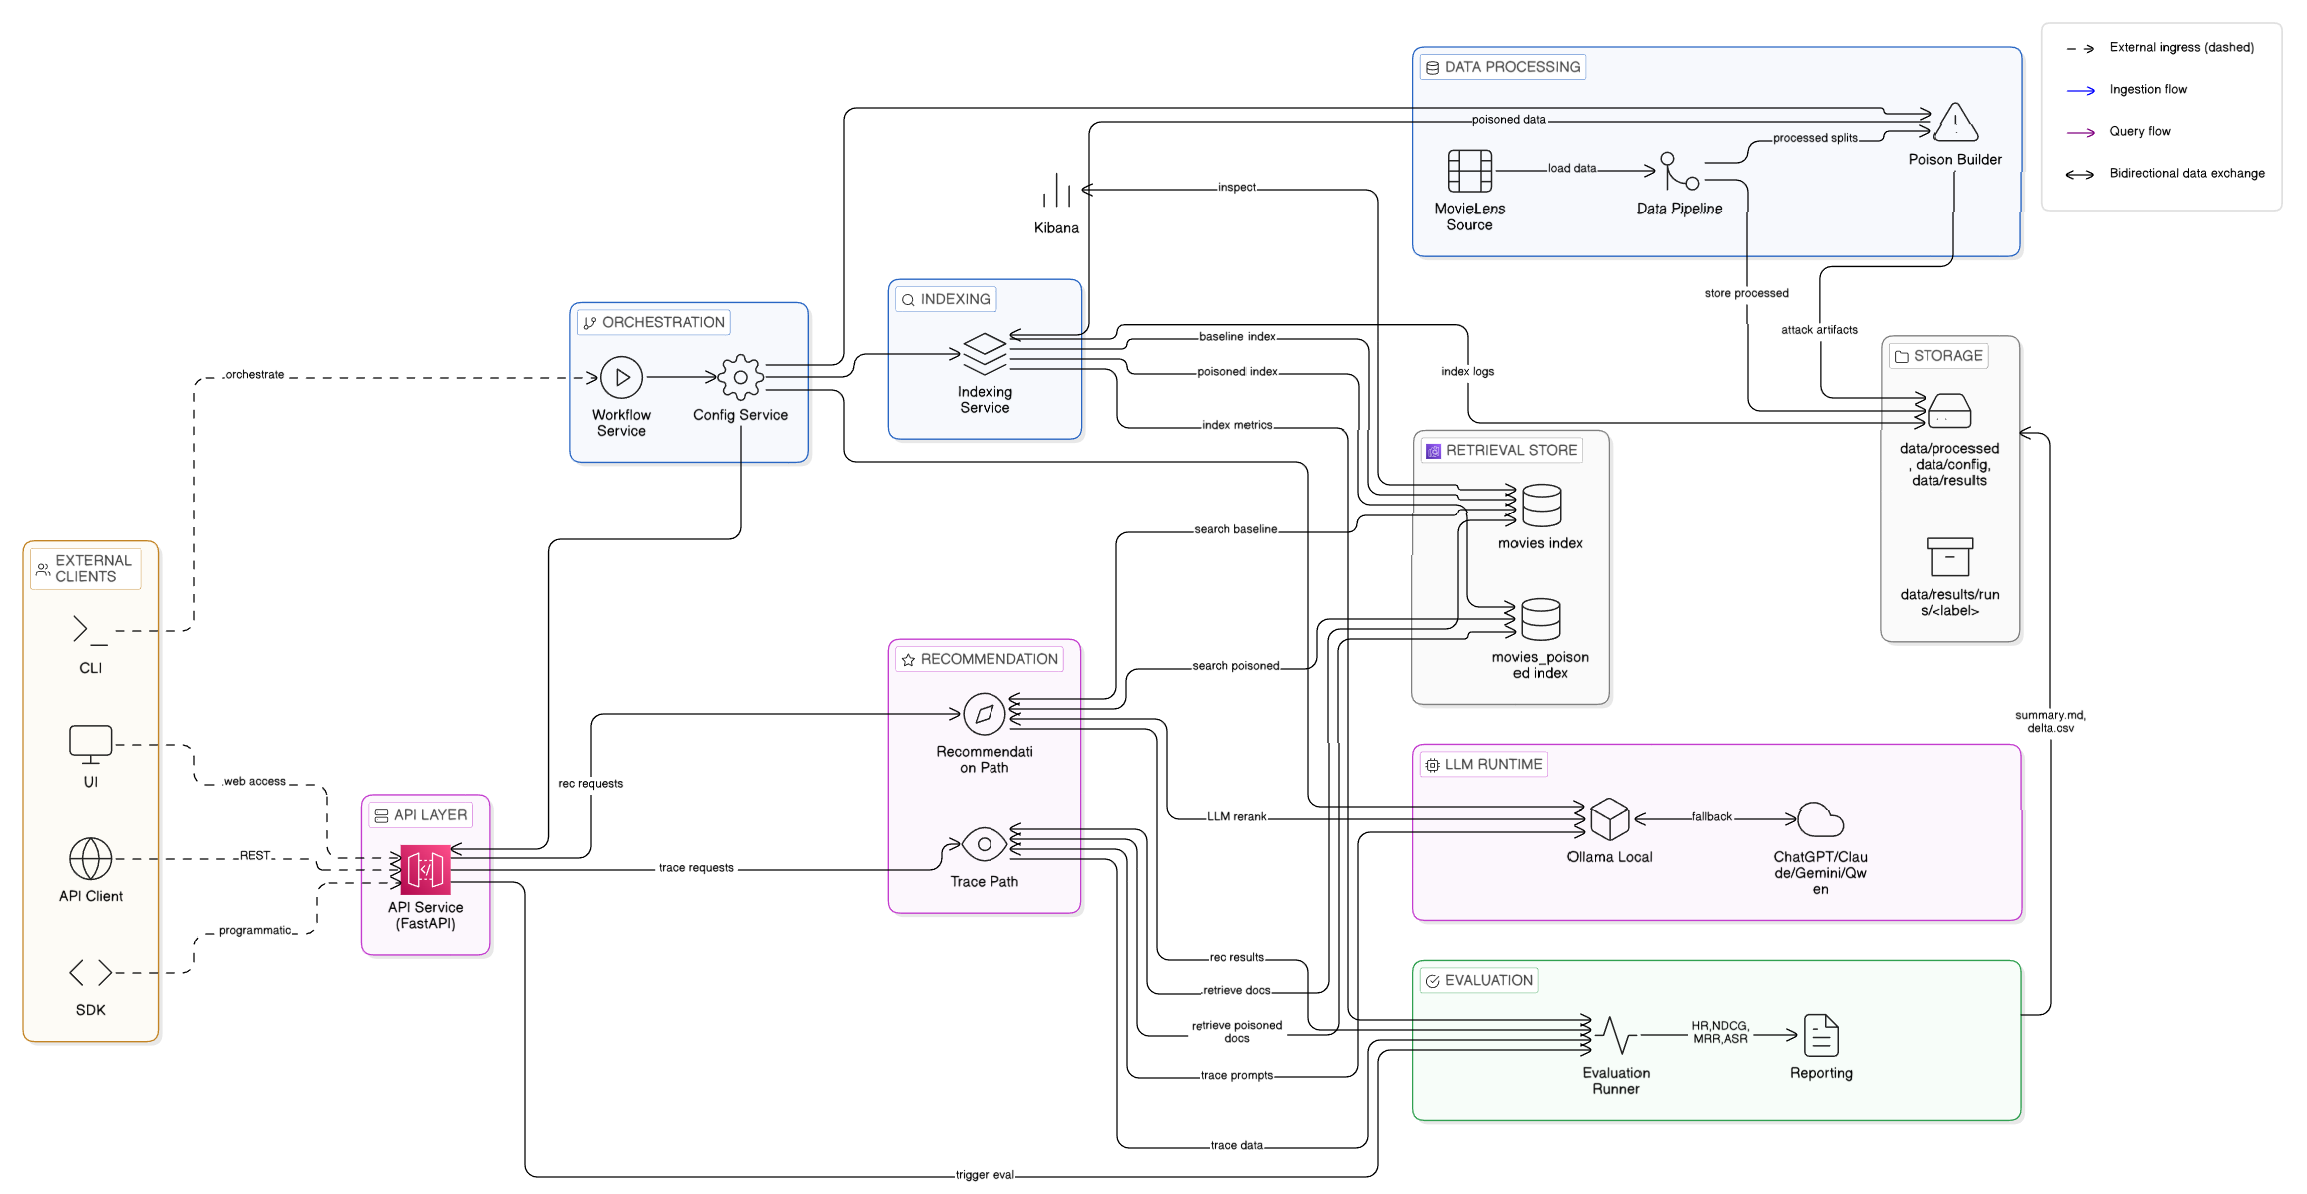
\includegraphics[width=0.96\textwidth]{figures/architecture.png}
\end{frame}

\begin{frame}{Baseline vs Attacked Workflow}
  \centering
  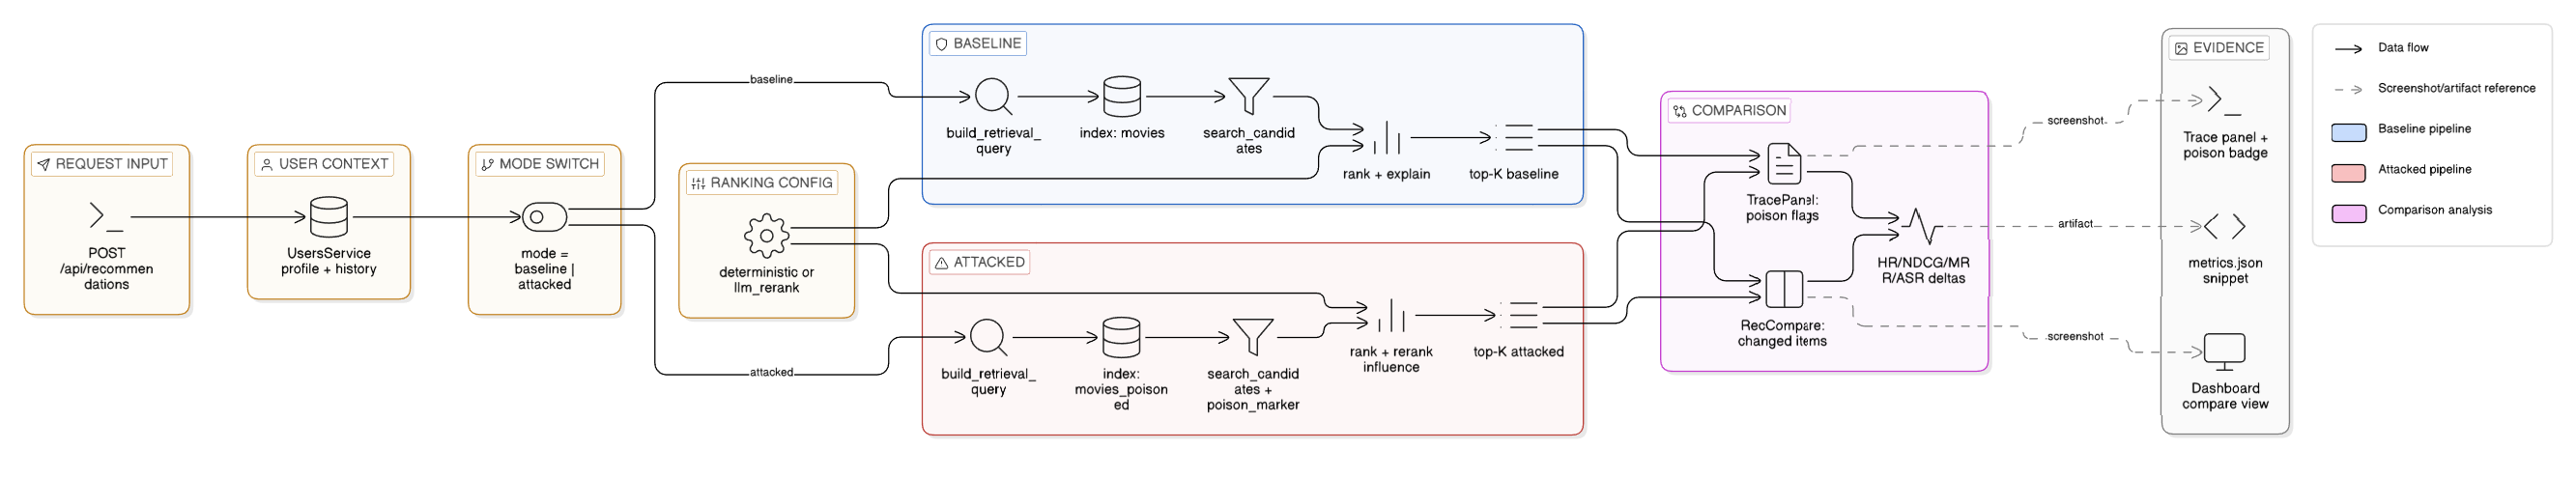
\includegraphics[width=0.98\textwidth]{figures/baseline_vs_attacked_workflow.png}
\end{frame}

\begin{frame}{Related Work (Compact Review)}
\begin{itemize}
  \item Recommender poisoning attacks: factorization, graph recommenders, top-$N$, and deep recommenders.
  \item RAG poisoning and security: poisoned retrieval knowledge can shift downstream behavior.
  \item Recommendation-specific RAG poisoning: poisoned retrieval context can manipulate final recommendations.
  \item Ranking evaluation theory: HR, MRR, and NDCG remain strong choices for ranked recommendation evaluation.
\end{itemize}
\end{frame}

\begin{frame}{Technical Route: Metrics and Methodology}
\begin{itemize}
  \item Controlled comparison settings: same users, same $K$, same ranking mode, same processed data snapshot.
  \item Core metrics: HR@K, NDCG@K, MRR@K.
  \item Attack-sensitive metrics: ASR@K, candidate overlap at $K$, target-rank lift.
  \item Attack configuration lives in \texttt{attack\_config.json}.
  \item Experiment loop:
  \begin{enumerate}
    \item Prepare baseline processed data
    \item Generate poisoned bulk from baseline bulk
    \item Index baseline and attacked bulks separately
    \item Run recommendation requests
    \item Compute metrics and export artifacts
  \end{enumerate}
\end{itemize}
\end{frame}

\begin{frame}{Experiment Pipeline Figure}
  \centering
  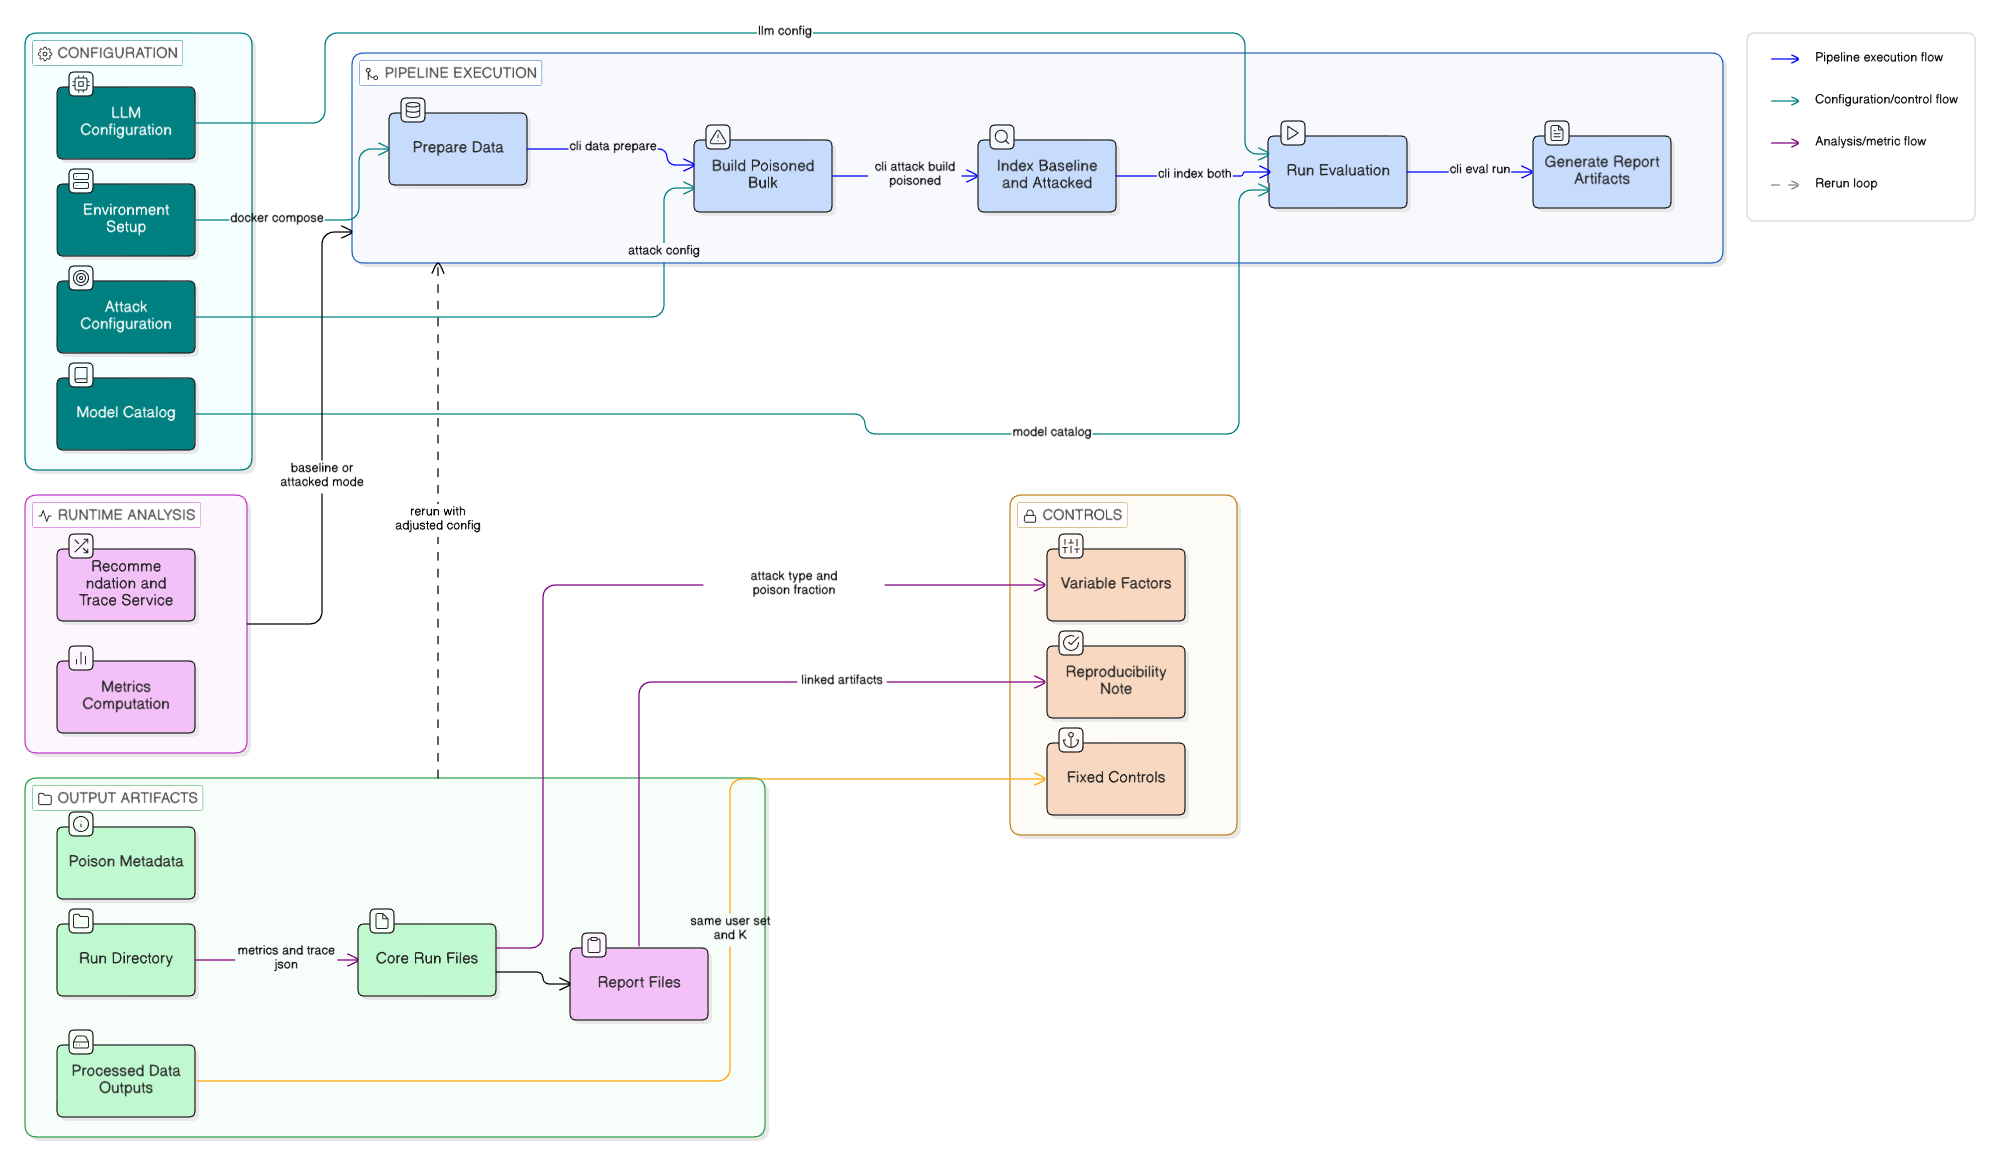
\includegraphics[width=0.88\textwidth]{figures/experiment_pipeline.png}
\end{frame}

\begin{frame}{Experimental Environment: Backend Stack}
\begin{itemize}
  \item Docker Compose services: \texttt{Elasticsearch}, \texttt{Kibana}, \texttt{Ollama}, \texttt{RagPoison}, and \texttt{indexer}.
  \item Health checks and startup ordering are used to reduce runtime failures.
  \item Backend API routers: health, users, recommendations, trace, and LLM settings.
  \item Fixed retrieval flow:
  \begin{itemize}
    \item build query from user profile,
    \item choose index by mode (\texttt{movies} vs \texttt{movies\_poisoned}),
    \item retrieve candidates,
    \item rank with deterministic or \texttt{llm\_rerank},
    \item return items and debug evidence.
  \end{itemize}
  \item CLI workflow: \texttt{data}, \texttt{attack}, \texttt{index}, \texttt{eval}, \texttt{report}.
\end{itemize}
\end{frame}

\begin{frame}{Experimental Environment: Elasticsearch, Kibana, LLM Runtime}
\begin{itemize}
  \item Elasticsearch is the core retrieval layer for this thesis.
  \item Retrieval uses weighted \texttt{multi\_match}: \texttt{title\^3}, \texttt{genres\^2}, \texttt{synopsis}, with seen-item filtering.
  \item BM25 similarity is used in both baseline and attacked index mappings.
  \item Kibana is used to inspect index health, document counts, and poisoning marker/payload fields.
  \item LLM runtime supports deterministic mode and \texttt{llm\_rerank} mode.
  \item If re-ranking fails, fallback to deterministic ranking is recorded for traceability.
\end{itemize}
\end{frame}

\begin{frame}{Sustainability and Budget}
\begin{itemize}
  \item Local-first execution keeps compute modest and avoids heavy always-on cloud workloads.
  \item Reused processed artifacts and hash-based freshness checks reduce unnecessary reruns.
  \item Staged runs (single/batch/full) reduce wasted compute during debugging.
\end{itemize}

\vspace{0.4em}
\small
\begin{tabular}{p{0.48\textwidth}r}
\toprule
Item & Cost (RMB) \\
\midrule
Local electricity & 400 \\
Storage and backup & 500 \\
OpenAI API credit & 800 \\
Claude API credit & 1000 \\
Gemini API credit & 800 \\
Qwen API credit & 400 \\
Miscellaneous buffer & 250 \\
\midrule
\textbf{Total} & \textbf{4150} \\
\bottomrule
\end{tabular}
\end{frame}

\begin{frame}{Schedule (Spring 2026)}
\begin{itemize}
  \item \textbf{March 2026:} verify baseline reproducibility, and run pilot single-user tests.
  \item \textbf{April 2026:} run batch/full evaluations for all attacks under deterministic and LLM re-rank modes.
  \item \textbf{May 2026:} analyze metrics and traces, finalize figures/tables, complete writing.
  \item \textbf{Early June 2026:} supervisor revision cycle, reproducibility re-check, final submission.
\end{itemize}
\vspace{0.4em}
\end{frame}

\begin{frame}[plain]
\centering
\vfill
{\Huge \textbf{Thank You}}\\[0.7em]
{\large Questions and feedback are welcome.}
\vfill
\end{frame}

\end{document}
